\chapter{Contribution}
In this chapter ..

In the following sections "Observable" is used to denote an actual RxJS Observable and also as a placeholder for any Reactive entity from RxJS or BaconJS in lack of a better term.

\section{Advancing the User Interface}
The User Interface (UI) is an important part of every application. A good UI helps the user focus on the task at hand by displaying the necessary information required for that task. For a Website this task may simply be to find gather information about the subject of the Website itself. An IDE usually provides many tools the user can use and reduce the manual work of the user by automating some steps of the development process. There are many factors that need to be taken into account when developing a new UI or changing an existing one. A UI should normally be designed to match the special use-cases the application was designed for while also keeping some familiar elements to guide the user. The main reason to keep a somewhat familiar look or have a certain part of the UI match what the user expects and knows from other applications in his domain, is that the user already knowns how to interact with familiar elements and does not have to learn how to use them from scratch. It is also important to consider some of the characteristics of human cognition. To explain them all in detail is beyond the scope of this thesis. To solve this type of problems if a main target of the Interactive Graphics Systems Group (GRIS) at TU-Darmstadt and many other groups world wide are working in this field. In the following paragraph we examine the changes to the UI of CRI we implemented in this thesis and the reasoning behind these changes.
  
\textbf{Reducing the cognitive load on the user}
The main goal of the changes to the UI we implemented in this thesis is to reduce the cognitive load on the user. If the user has to concentrate and search for information they need to achieve their task and not having them presented in an easy to find and understand manor, half of his attention is already occupied. It can not be used to work on the task and achieve their actual goal.

The first change we introduced to reduce the cognitive load on the user is to move some input elements to a menu that is displayed at the top of the CRI's UI. Nearly every desktop application and many Websites (e.g. http://reactivex.io/rxjs/, Windows File Explorer, Eclipse, Microsoft Paint, Adobe PDF Reader and many more) use a menu at the top of the UI. This adds structure and also removes many buttons from the normal working space which can then be used to display more relevant information. The user knows that the buttons are in the menu and searches though it on demand. The buttons hidden in the menu bar do not require space or attention by the user at other times, except for the space required by the menu itself. We examined our own usage frequency, how often we use a certain input element, and estimated the tasks that include the input element to determine which elements should be part of the main UI and which should be hidden in a menu (or closeable panel for inputs other than buttons). We found that we rarely used the \emph{Reset}, \emph{Download} and \emph{Pause/Resume} buttons. The latter was used most among them and since CRI does not actually have loads of buttons yet, we decided to place it directly in the menu bar instead of moving it into the sub menu used for the other rarely used buttons. The \emph{Pause/Resume} button is also the only one of those buttons used in a normal workflow, i.e. in the special case of working with Rapidly updated Observables (see section \ref{sec:RapidlyUpdatedObservables}) it is used regularly to counter performance issues or focus on a specific part of the execution.  %TODO: maybe add screenshot of menu
The other buttons of the UI are part of a specific feature of CRI and can not be moved away from other elements that belong to the features. These features from left top to bottom right are the Instrumented Files list, History Queries and the navigation through the results, Reactive Breakpoints, Search, History Navigation and the Dependency Graph. The Dependency Graph and History Navigation are closely tied together and represent the main part of CRI. They are the working area where the focus of the UI should be. The other features are complementary to them support the user ins examining their content. Although CRI can be used effectively without History Queries and Reactive Breakpoints they can help the user in almost any task. Reactive Breakpoints may even be mandatory to discover some issues with an application that otherwise could not be detected without a much greater effort (similar to normal Breakpoints in traditional IDEs). While the Dependency Graph with its History is just another way to provide an abstract representation of Observables and Dependencies then the Marble Diagrams used in RxFiddle, Reactive Breakpoints are currently exclusive to CRI. In conclusion, History Queries and Reactive Breakpoints should be a permanent part of the UI, therefore we decided to keep them where they were positioned in CRI2 - above the History Navigation. The Search feature is not as important in most tasks. The highlighting of a specific node, its Dependencies or Dependents is only useful for applications with large Dependency Graphs. Small graphs can easily be searched for the required information manually with one look. Therefore the Search feature could be moved to a closeable panel that is only opened on demand. The search implemented in most IDEs opens when the user presses CTRL F or clicks the search button in the menu. The reason we did not move the feature to a closeable panel yet is simply that the area of the UI where the History Query and Reactive Breakpoints input elements are placed provides enough space (with standard screen resolutions sizes for desktop computers) to keep the Search there as well. With the current UI the space is otherwise left empty. However as soon as these parts of the UI change or another feature is introduced, the Search should be moved to a closeable panel. The remaining feature is the Instrumented Files list. It is used as a scoping feature to select which files should be instrumented. For small to medium sized applications the list of files will normally include all relevant JS files and will not be changed at all. It is therefore reasonable to move it from the main UI to free the space that could then be used to increase the size of the Dependency Graph canvas. After examining the outcome of this change we found however, that in case the user switches to another application that requires other files to be instrumented or forgot to include a JS file in the list, it can be really difficult to detect the reason why the Dependency Graph is not showing the expected result. If the Instrument Files list is moved from the main UI, the user may loose track of the fact that not all JS files are automatically instrumented or, if they decided to instrument only a subset of JS files as a filtering measure, that the >filter< is still in place. It is also easier for new users to comprehend the need to select files for instrumentation if the list is part of the main UI. This could be mitigated by adding a dialog informing the user at the first start of CRI, but for this reason in addition to the reasons mentioned above we decided the benefits outweigh the downside of a small part of the UI being occupied by a rarely changed input. Therefore we kept the Instrument Files list at the top of the UI and also added a red border around the text input as an validation error in case the list is empty to help make new users aware of the missing input.

To further decrease the cognitive load when working with CRI, we removed any text from nodes and their tooltips that do not carry any value. The less text there is on the UI, the less as user has to read to find the information that they require. This is most significant for the \emph{Method} field in the tooltips since most Observables do not correspond to a method and the field therefore is empty for most nodes. The \emph{Value} field is usually set, but if there is no value, there is no need to keep the label for the field. The same information is available to the user if the label for \emph{Value} is simply omitted in that case.
It is however important to display values that explicitly denote an \emph{empty} value like \emph{undefined}, \emph{null}, or -1 (for a value that carries positive numbers if it is set). The \emph{Name} field is also not set for every node. Figure \ref{fig:Nodes} shows an example of nodes from CRI2 with all field as well as nodes from the current version.

\begin{figure}[!h]
	\centering
	\subfloat[CRI version 2.0]{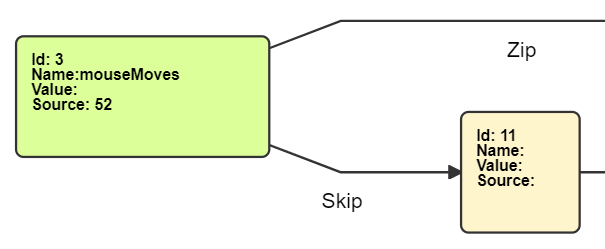
\includegraphics[width=0.4\textwidth]{gfx/NodesCRI2.png}\label{fig:NodesCRI2}}
	\hfill
	\subfloat[CRI version 3.0]{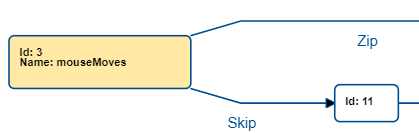
\includegraphics[width=0.4\textwidth]{gfx/NodesCRI3.png}\label{fig:NodesCRI3}}
	\caption{A sample of nodes before and after the changes introduced by this thesis.}
	\label{fig:Nodes}
\end{figure}
%TODO: casing of \emph{Named} node and dependency
Another important aspect to consider is if to display a field on the node directly or in the tooltip. The same principle that applies to general elements of the UI applies here as well. Only values that are necessary to always have present without the need to open every tooltip should be displayed as part of the nodes. We evaluated for each field where it should be located regarding this criteria. The \emph{Name} is important to identify relevant nodes, including those depending or dependent on a \emph{Named} node. The \emph{Id} is required to add Reactive Breakpoints and to identify nodes without a name from one step to another in case the nodes are repositioned due to a new edge being added. The \emph{Value} is normally the property at which developers can see if the JS code of the application works as intended. E.g. an Observable is expected to have a specific value at some point in the execution. The developer can also observe a value passing along the chain of dependencies. For these reason the fields \emph{Name}, \emph{Id} and \emph{Value} should be always displayed, as long as they have a value, as part of the node.
The \emph{Type} should be hidden in the tooltip, because often what type of Observable the framework uses internally does not matter to the developer. E.g. in most scenarios for RxJS there is not difference between a FromEventObservable and a basic Observable. The information should however, be still present in the tooltip and not omitted completely, because some types of Observables do behave differently than others e.g. RxJS Subject vs Observable. The source code position labeled \emph{Source} is also just used in few special tasks. On example is the user wanting to find the source code corresponding to a node in the graph to modify that code or inspect it further. The \emph{Source} should therefore be displayed in the tooltip rather the nodes themselves. The field \emph{Number of Updates} was introduces by this thesis as a way to detect bottlenecks and help identify nodes that cause the generation of a huge amount of steps through excessive value updates in CRI. It is based on the Time Profiling feature of the Reactive Inspector \cite{ReactiveInspector}, but for now only provides the total number of updates on a node instead of detailed timing and value evaluation information. It is only useful for the purposes mentioned above and therefore should not be displayed on the nodes themselves.

An important cognitive task that a user has to do often while using CRI is to track changes between steps in the Dependency Graph History. To track these changes is necessary to understand how the graph is constructed or to track value updates traveling along a chain of dependent Observables. It is however not always trivial since the rendering engine \emph{D3.js} \cite{D3JS} used by CRI sometimes moves nodes and edges around to better fit the available space. To help the user with this task, the previous version of CRI already highlighted the nodes that were changed for each step in which a node was changed. We extended this feature to also highlight edges that were updated or added to further decrease the manual searching process. Another feature we added to the UI is a button that hides the tool section of the UI - everything except the menu, History Navigation and Dependency Graph - to allow the user to reduce distractions and free up additional space if they want to focus on the manual examination of the graph and its History. The button is located at the top right corner and has a small arrow icon instead of a text label to reduce its required space in the UI. The option to hide the tool section is especially useful when working with a small screen or a big Dependency Graph. Another button we added to the UI, as part of the menu, was a button to reload the inspected page and therefore the Dependency Graph as well. We discovered that reloading, was already part of the usual workflow by pressing CTRL F5 and decided to add a button that allows user to achieve this without being aware of the short cut. An example workflow in which a reload can be used is to create a breakpoint for \emph{dependencyCreated} or \emph{nodeCreated}, and then reloading the application to actually hit the breakpoint.
As figure \ref{fig:Nodes} shows, we also change the colors used in the CRI UI. The node that was changed in the currently viewed step was highlighted by using a red border in the previous version of CRI. The color red is a signal color normally used to show that immediate attention is required or to show that an error has occurred. In traffic signs and lights the color red is used to signal cars to stop or to be aware of dangers. Therefore we decided to remove it from the normal workflow of CRI. Highlighting the current node is important for the user to immediately identify the change, but it does not require the users full attention the whole time. It also neither represents an error, therefore the increased cognitive load on the user is unnecessarily. The combination of red and green (\emph{Named} nodes) is also problematic for some users with vision deficiency, although as the green is a very bright shaded they should still be able to distinguishable the border on a highlighted \emph{Named} node. Because of these reasons we decided to use blue with light orange as the highlighting that has less contrast between the two shades, but still enough to not void the highlighting. To this purpose we chose a shade of blue and selected the colors for nodes, edges and highlighting from suggestions provided by a color scheme designer \cite{Paletton}. We chose to keep the text color black, because it is the most used color for text in general and is easy to read on most colored backgrounds. The nodes that do not correspond to a named variable were left without a background to further reduce the cognitive load. The brain is trained to ignore empty spaces therefore making the text and named nodes appear more important.

Another change we introduced to the UI of CRI was the automatic reloading of the graph if the Instrumented Files list changes. This does not reduce the cognitive load on the user, but removes a redundant click on the reload button. It is not very useful to change the list of instrumented files without restarting the inspected application and the recording. If the application is not reloaded automatically it will also confuse the user that their change does not have an immediate effect. %TODO rephrase last sentence
	
\section{Connecting abstract graph with JavaScript code}
Nodes in the Dependency Graph that correspond to Observables that are directly assigned to variables provide developers with some form of context. A \emph{Named} node can be used as an anchor to identify the node itself as well as other nodes up and down the chain of dependencies. It helps the user to separate parts of the Dependency Graph that are relevant for the piece of code they want to examine and parts that are currently not relevant. Without any orientation it is very hard to interpret a shown Dependency Graph. The user can still try to identify nodes by their values or the values of their neighbors, but these values can be missing at certain stages of the application. This all boils down to the issue of connecting the abstract representation of the applications Observables provided by the Dependency Graph with the actual JS source code responsible for those Observables. If an error is detected by examining nodes in the Dependency Graph, the user still has to track down which lines of code are responsible for the issue in order to change them. As mentioned above, \emph{Named} nodes solve this issue in a way, but not all Observables created during runtime are assigned to variables. In fact, even if possible, this is not at all desirable. To the result of each function in a chain of functions to a variable negates most of the benefits of using chained functions in the first place. If the variables are not used by multiple lines of code and are just introduced to support the debugging tool, most of all the disadvantages of \emph{do-debugging} apply as well. We therefore evaluated several possibilities to provide nodes that do not have a corresponding variable with additional details that help provide some context to the user. A very basic form of context was already present in the previous versions of CRI in form of the source code position information. This information was however, not very accurate in case of chained functions, because only the start of the source code position information provided by Jalangi was used. In case of chained functions the source code position actually spans a block that may consist of multiple lines of source code. In addition information provided did not contain the name of the JS file to which the position belongs. Another downside of this approach is that to look up the source code in another tool apart form CRI and switching back to CRI to check the position of the next node is very cumbersome to execute for more than a few nodes. The developer should be able to easily switch between source code inspection and examining the Dependency Graph, because not all issues can be found in either of them when used alone. For example, if there is an issue in a lambda function, a user can not find this issue directly in the Dependency Graph. They can only see the result in node values that do not match the values that they expect with the original intention of the code in mind. The main difficulty to achieve this by showing actual source code instead of just the position information is JS code that is used during runtime is instrumented with Jalangi to enable a detailed analysis. Jalangi instrumented code is very hard to read as is shown in listing \ref{lst:Instrumented}.

\begin{lstlisting}[language=JavaScript, caption={Example of RxJS code.},label={lst:Instrumented}]
$sonWallet = J$.W(593, '$sonWallet', J$.F(585, J$.I(typeof $ === 'undefined' ? $ = J$.R(569, '$', undefined, true, true) : $ = J$.R(569, '$', $, true, true)), false)(J$.T(577, '#wallet-son', 21, false)), J$.I(typeof $sonWallet === 'undefined' ? undefined : $sonWallet), true, true);
$fatherWallet = J$.W(625, '$fatherWallet', J$.F(617, J$.I(typeof $ === 'undefined' ? $ = J$.R(601, '$', undefined, true, true) : $ = J$.R(601, '$', $, true, true)), false)(J$.T(609, '#wallet-father', 21, false)), J$.I(typeof $fatherWallet === 'undefined' ? undefined : $fatherWallet), true, true);
\end{lstlisting}

For example "J\$.W" signals the analysis engine that a write operation is executed when the function is called. This makes it unfeasible to directly show the instrumented code to the user. In addition to being very hard to read, the instrumentation of the source code is an implementation detail of CRI and should not be exposed. Additionally the code position retrieved from the Jalangi analysis corresponds to the position in the original source code without instrumentation. Note that the JS code that is used during runtime is also dynamically loaded and therefore can not be navigated to out of the box with Chrome DevTools navigation API. Although this is mitigated by adding "//\# sourceURL=" with a custom URL to the bottom of a script. Since this shows the Jalangi instrumented source code that is not useful for a normal user, we decided to tie this to a new option called \emph{CRI Developer Mode} that can be enabled in the options page of CRI. The different approaches discuss in the following section are designed to enable a user to use both the abstract representation and the source code in tandem.
	
\subsection{Evaluated possibilities of displaying source code}
\textbf{Using the \emph{chrome.debugger} API}\\
One possible option is to use the \emph{chrome.debugger} API to open and navigate to the corresponding position of a node. It is easily possible navigating to a line number in a file, if the actual file URL, which can differ for dynamically loaded scripts due to many factors, is known. For the reasons explained above, navigating to the instrumented code is not desirable. A non-instrumented version seems to exist in Chrome's \emph{Source} windows as a dynamic script, but it is not actually used at runtime. This approach provides the user with syntax highlighting through Chrome and other features like search with regular expressions. They could also inspect the whole code of the application, not just the piece of code corresponding to a single node if required. The downside of this approach is that the user needs to leave the UI of CRI to access the source information. For a single node this is not an issue, but it is really cumbersome to inspected the source information of multiple nodes, even if the navigation to the position is automated. It is not possible to highlight the code block that corresponds to the inspected node, which would be especially useful for Observables corresponding to the middle of a block of chained functions. The start and end of the block would have to be manually searched for. Another downside that most likely confuses the user, is that some features of Chrome's DevTools can be used but others will not work and there is no way for CRI to display this disparity. Due to the code shown to the user not actually being executed, all features specific to runtime interaction like breakpoints, direct code evaluation or watches will not be usable although a user familiar with Chrome's debugging capabilities will most likely expect them to work properly. A modification of this approach is to display the code in another IDE than Chrome. As some modern IDE's provide a featured to navigate to a functions declaration (in WebStorm called "Go to declaration") which is more scalable than using a String based search for enterprise sized applications. Although this feature is not available in Chrome, having the user install another IDE and use that in parallel with Chrome will increase the dependencies of CRI and the development effort coupled with that dependency while still suffering from all the downsides of this approach explained above.\\
\textbf{Using an integrated lightweight IDE}\\
Another possibility is to use a file viewer that is opened for example as a closable panel to show the full source code. Depending on the implementation this approach can provide full customization of code presentation to the user. In theory, advanced syntax highlighting (syntax highlighting based on the usage and structure of functions like WebStorm does to detect >classes<) could be applied. It is also possible to highlight Observables in the source code while the user hovers over the in the Dependency Graph or even permanently coloring the source code based on the abstract representation. The main problem of this approach is the development effort required to achieve a viable implementation. There is no library available, that we are aware of, that provides the needed functionality and customization options. To develop such a library ourselves requires nearly the same amount of work needed to develop a traditional IDE for JS since it basically is a lightweight JS IDE displayed in a panel of CRI. Another issue with this solution in addition to the required development effort is that nodes that are close in the Dependency Graph, because they share a dependency do not necessarily correspond to code that is located in close proximity of one another. The code may even be split over several JS files in extreme cases which requires additional view options by any lightweight IDE apart from just showing one JS file.\\ %TODO: search for 'web'
\textbf{Mirroring interactions to a non-instrumented copy of the application}\\
An approach that is possible in theory, but will not withstand a detailed evaluation is to mirror any interaction to the inspected application to another version of it. The idea is to have one application with instrumented JS files, and one where the JS files are not instrumented. This would enable CRI to use another approach like using the \emph{chrome.debugger} API to display the actual source code used at runtime while retrieving analysis data from the instrumented mirror application. It enables the user to use every feature of Chrome or another IDE when debugging JS. The problems introduced by copying the entire application and mirroring any interaction to it go, however, far beyond the doubled resource consumption. One mayor issue is the actual recording of user interactions to the original application. There are many tools like Katalong Studio \cite{Katalon} using Selenium \cite{Selenium} that can be used to record and replay interactions to a Web application. These tools are often used to automate the testing of Web applications. Most of these tools are therefore designed to ignored certain aspects of interactions like positioning of elements to make the tests more robust against small changes. Although there are some tools that use pixel positions to record and replay interactions. We could, however find not one tool that records mouse movements and replays them exactly. It is possible to develop a solution oneself, but the mentioned tools solve many issues like always replaying with the exact same screen resolution that is especially important if the layout of the applications UI reacts to different screen resolutions. Another issue with replaying interactions to the copied Website are security restrictions imposed by Chrome (and other modern browser) itself. Chrome restricts some special interactions a user can execute to not be mimicked by a Web application of Chrome extensions to shield users from attackers that use a custom extension or Website to influence Web applications outside of their own domain. An example of these restricted interactions is the using of Chrome's Context Menu or the operating system's Clipboard. The reasoning to restrict both are similar and are due to the fact that these features can be used to breach boundaries otherwise monitored by Chrome itself or in case of the Clipboard by the operating system. Since these interactions can not be mimicked, it is impossible to replay them on the mirror Web application. This voids all other attempts to replay any other interaction, because the two applications will desynchronize. The danger of the two applications becoming desynchronized can also be created by Observables or JS code in general being time sensitive. For example an Observable or function that is scheduled to be executed or updated every few milliseconds and has any side effect like increasing a value by one every time the execution happens, needs to match exactly to produce the same result on the mirrored application. This also includes any JS code that is execution order dependent. The same execution order must be maintained, which is especially hard for asynchronous code even though JS's runtime is event-based \cite{EventBasedJS} and does not actually execute code in parallel. In summary, any code dependent on the order of execution or anything timing related has to be mimicked exactly to keep the mirror in sync with the original application, which can not be guaranteed for all possible applications in a normal environment. \\
\textbf{Source Code Tooltips}%TODO: explain chained functions somewhere
%TODO: lambda function definition
%TODO: make sure there are not duplicates in Implemented Solution.
The solution we decided to implement is an extension to the already present tooltips for the nodes. The tooltip for a node that the user hovers over with the mouse pointer changes to a short snippet of source code, corresponding to the node with a few lines of code before and after the relevant code as orientation, that opens if the user presses the CTRL key. For details of the implementations see the next section. This approach however has some limitations. If the node belongs to an Observable at the end of a long chain of functions or a lambda function is used that covers several lines, the code piece may actually be to long to show in a tooltip. If the code is not wrapped properly the code will also be hard to read in a tooltip due to the limited space. In addition it is also not possible to use any kind of tool inside a tooltip like for example searching. As the tooltips are relatively short, this issue is not to serious as the code snippet can quickly be read altogether. Another limitation of this approach is that it is not possible to view the full source code. Since the user can not change the source code in CRI either, they have to switch to another tool anyway at some point. For now the Source Code Tooltips do not provide syntax highlighting and, if added in the future, it is important to note that syntax highlighting of short snippets is not very effective in JavaScript. Since JavaScript is dynamically typed language, it is necessary to take usages in other areas of the code into account to correctly highlight language elements beyond reserved keywords. The usefulness of Source Code Tooltips is also greatly decreased, if a normal function instead of a lambda function is passed to an Observable Operator. Some other patterns like using callbacks that are not realized as lambda functions or functions that create other functions also have the same issue. An example of this is shown in listing \ref{lst:NonLambdaCallback}.

\begin{lstlisting}[language=JavaScript, caption={Example of using a creation function in RxJS.},label={lst:NonLambdaCallback}]
function createFunction(add) {
return (value) => value + add;
}
let fatherWalletValue = sonWalletValue
.map(createFunction(10));
\end{lstlisting}

The source code corresponding to the \emph{Named} node "fatherWalletValue" ranges from line 4 to 5. If the function declaration is not directly placed nearby and therefore shown in the tooltip as well, it is not possible to view the implementation of "createFunction" in the UI of CRI.
The greatest benefit of using Source Code Tooltips is that they compliment the Dependency Graph very well. A user does not have to leave CRI to view the corresponding source code and the abstract representation is still the focus of CRI. The tooltips solve the issue of providing additional details for nodes that do not have a corresponding variable name. In fact, they provide additional information for these nodes as well. Using tooltips also has the advantage that they are easy and fast to open and close again. Therefore the user is able to inspect several tooltips in short sequence. This helps them to find and remember nodes without a corresponding variable name between multiple uses of CRI by other means than remembering the Ids.  The Ids will also change if the user modifies source code that adds new nodes to the Dependency Graph or changes the order of existing ones. Another benefit by using Source Code Tooltips is, that we are able to highlight the exact source code block responsible for a node even within a chain of functions. This is similar to the possibilities when using a  custom lightweight IDE. In contrast to using another full fledged IDE however, using tooltips inside CRI does not introduce new dependencies. Another very important feature of using tooltips is that they do not require additional space in the UI. Using a panel that opens on demand as a pop up or as part of the UI would result in a resize and movement of other UI elements or overlap parts of the UI until it is closed manually. Instead, the normal tooltips open when a user hover over a node and will be replaced when they hold the CTRL key. If they release the key or move the mouse away from the node, the tooltips will change back or close automatically. This fits well in the already existing workflow of inspecting several nodes with the mouse pointer and is in our opinion very intuitive to use. There was, however no User Study conducted as part of this thesis to verify that this is true for the majority of users. We chose this approach based on the benefits it provides, even though there are some downsides that will require additional development effort to overcome in the future.
			
\subsection{Implemented Solution - Source Code Tooltips}
In this section we explain the implementation of the Source Code Tooltips in detail. To retrieve the non-instrumented source code necessary to show in the tooltips, we store them in a dictionary before executing the instrumentation. To provide the correct source code, we first extended the Jalangi framework used in this thesis. As explained in chapter \ref{ch:State of the Art}, the used Jalangi framework is not actually the full Jalangi, but just an in-browser version developed for a single demo. It therefore does not support many features of the actual Jalangi. One of these features is the required JS file names that are not included in the position information provided by the demo Jalangi. We therefore decided to implement an ad-hoc solution to retrieve the filename. There is no way to determine the source JS file inside the Jalangi analysis, because the Jalangi sandbox object is shared by all JS files and the information is not submitted as a parameter to any of the analysis methods. The only solution with minimal changes to the used Jalangi framework, which is desirable if it is ever updated, is to replace the J\$ object, with a shallow copy of the original J\$ object. The copy provides the required information and then calls the original. The "W" function of Jalangi is responsible to intercept variable assignments and is used to link nodes to a corresponding variable name. We extended this function and any function responsible for passing the recorded information to the analysis engine to accept the filename as an additional parameter. This replacement is done for every JS file with the corresponding filename. However, since the Jalangi object is quite large, we decided to exclude in-line JS scripts directly embedded within the HTML. In-line scripts are often very short and can not be taken out of their context in the HTML easily. Otherwise it would be possible to collect every in-line script and add them to an external script that is then instrumented and modified with the replacement J\$ object. Therefore one copy for every in-line script is necessary. The shallow copy from JQuery that we used, duplicates only references and not data, but for large objects with many functions this still has a performance impact if done repeatedly. But there is actually no downside in omitting the in-line scripts from the Jalangi extension, as we simply know that any node with source position information that do not specify a file name to which the position belongs stems from an in-line script. The file name of these nodes is labeled as \emph{html}.\\
With the implementation so far, only nodes with a corresponding name will have a Source Code Tooltip, because only variable assignments were reasonable to capture in the previous versions of CRI. We therefore extended the analysis engine (located in jalangi-analysis.js) to also intercept function invocations. This enables the recording of source code position information for functions and their parameters. We only check the return value of the intercepted functions if they are an Observable, because the function arguments either are not Observables, or they are created by a call to the Reactive Framework and should already have been recorded. To retrieve the file name information as well we extended the corresponding functions of the J\$ object similar to the extension of the variable assignment interceptions. With this implementation it is possible than an Observable is recorded multiple times for the same node, for example if a node is assigned to a variable inside a function and then returned as the result. In this cases it is important to always use the position information intercepted from the variable assignment. The reason for this is that if the node in the Dependency Graph has a name from a variable, the Source Code Tooltip should always show the assignment of that variable in order to not confuse the user. Note that since we retrieve the source code position information from the Jalangi analysis, the Source Code Tooltips will not work for nodes that stem from JS files that are not selected for the instrumentation.\\

We made several additions to the UI of CRI in order to show the Source Code Tooltips in the way described above. The class TooltipManager (located in tooltips.js) handles the creation and displaying of tooltips for all nodes in the Dependency Graph. It adds the UI events used to switch out the tooltips and requests the code needed to construct the Source Code Tooltips from the instrumentation script if the tooltip was not opened before in this step for that specific node. The used tooltip library tipsyJS \cite{Tipsy} that was used in previous versions of CRI is no longer actively developed. We still decided to continue using it, because it provides a simple way to swap out tooltips as it accepts functions for any of the options passed as parameters to the library. However we had to modify the library to include a fix for a rendering issue that was already submitted as a pull request to the GitHub repository of that library but not accepted due to not being actively developed anymore. To enable the capturing of keyboard events for the Dependency Graph it is necessary to explicitly make the containing HTML element focusable. This is done by adding a \emph{tabindex} attribute. Since the container also needs to have the focus in order to receive the keyboard events, the container is automatically focused when the user moves the mouse pointer over the Dependency Graph. The mouse events used to open or close a Source Code Tooltip of a node are registered when the user hovers over the node and removed when the mouse leaves the area of the node. We also chose to give the user a visual clue if a node has a Source Code Tooltip. This prevents users having to probe each node if a Source Code Tooltip is available. The border of nodes that can not be linked to a source code position is therefore displayed faded. We chose this specific visual representation, because having no Source Code Tooltip means the node does not provide any context information and the normal tooltip will most likely also not provide any valuable information. One could argue that the Location information could now be omitted from the normal tooltips as well, but it is currently the only way for the user to see from which JS file the node originated, since Source Code Tooltips currently do not show the filename. However this may be changed in the future.
	
\section{Rapidly updated Observables}
\label{sec:RapidlyUpdatedObservables}
In this section we discuss the difficulties when handling applications with rapidly updated Observables and our approach to increase CRI's ability to cope with them. If the value of one or more Observable is changed rapidly, each change will result in a new step in the Dependency Graph's History. Observables that are for example created from timers, mouse movement or a network connection submitting messages change their value very often in a short period of time. The previous version of CRI is not able to handle rapidly updated Observables well. For a detailed performance comparison see chapter \ref{ch:Evaluation}. However there were two features added to CRI that enable the user to still use CRI with rapidly updated Observables to some extend. One feature is the option to pause the recording and resumed it at a later time. This feature is useful for applications that exceed the limits of CRI slow enough for the user to click the \emph{Pause Recording} button. The user can then examine the recording up to this point without any issues related to performance. This is due to the fact that any user interaction is slow enough for CRI to handle, while steps may be generated by the thousands in the same period of time if the recording is not paused. The other feature that was added is the ability to exclude certain nodes form the recording process, although this is cumbersome to do. The user has to detect and remember the Ids of nodes that are being updated rapidly and then add these Ids to a list located on the options page. This ad-hoc solution can still be useful in certain cases, but in others the full exclusion of a node will cause errors in the recording process. In the following we explain the increased demand on resources, the steps implemented to increase performance in this thesis and the limitations of the UI in handling these type of Observables in general. 

\subsection{Difficulties and previous approach}
Not only does the generation of hundreds of steps decrease the expressiveness of each individual step, with some exceptions, but it is also very demanding on computational resources. Messages between Content Scripts, Background Scripts and the extensions panel have to be transmitted in addition to saving the Dependency Graph's History. This also increases the number of rendering operations of the graph itself which requires a lot of size and position computations. If the computational effort exceeds the capabilities of Chrome and the underling system, CRI and sometimes even Chrome itself will stop working. There is a threshold regarding the minimum time span between individual updates that if undercut leads to CRI crashing at some point of the execution. The reason for this is the accumulation of requests if more requests are submitted, for example to the Chrome message or storage API, than requests are processed. Over time the resource demand on scheduling requests and managing the JS runtime's event queue increases beyond the available computation power. In this case the UI becomes unresponsive and Chrome will eventually terminate the extension. In the remainder of this thesis we will refer to this type of performance issue as \emph{request buildup}.
The steps that are often still significant to a user belong to the start of the History. They usually contain some form of setup phase, were Observables and their Dependencies are created, but there are no values submitted to them yet. An example of this is visible in many of the test applications, as value updates will not occur until the user starts using some form of input element. These steps can still be examined and provide valuable information that is not value update related about the created Observables. However the setup phase is not present in each Web application. If the application does not have a setup phase, the History becomes hard to examine. Even if there is a setup phase some parts may be implemented with something like the \emph{Lazy Loading} Pattern \cite{Lazy} in which the creation of Observables will just happen on demand. There may also be no setup at all. It is possible to create Observables dynamically - i.e. the type or dependencies used are a result of some form of computation or configuration - which will not necessarily happen at the start of an application. Another case in which the History becomes hard to examine for a specific task is if the application has multiple busy phases. Such an application may wait for some message from an external component that results in many computations and updated observables. Since the History does not provide an actual time line and will show steps in a linear sequence these busy phases become very hard to identify and distinguish. 
Another difficulty that stems from the \emph{Pause/Resume Recording} features, is that it results in a broken History. There is no visual feedback in the History Navigation that signals the user a pause has happened. If the recording is paused and later resumed, the steps before and after this gap are not sequential anymore, event though the History indicates the contrary. After the recording was paused, the Dependency Graph will actually show a false image of the variables as their value may differ from the actual variables in the application. This difference only persists until every node is updated once again, but if an Observable or Dependency is created during the pause, it will not be visible at all. The later is somewhat intentional for excessively, dynamically created Observables discussed in section \ref{sec:DynamicallyCreated}. But this still leaves the user to remember at which step they paused the recording or they will get confused if they examine the Dependency Graph while stepping over the gap.
	
\subsection{Reworking the Dependency Graph History}
%TODO: we used the local storage instead of the session storage because Chrome allows for larger data and reset it everytime it becomes void due to closing CRI or reloading the graph
To reduce the computational resources required to record the Dependency Graph's History and implement a more sophisticated storing mechanism, we reworked the previous implementation. The History records every change to the Dependency Graphs as a new step. While previous versions of CRI stored the whole graph for each step inside an array for simplicity. This means the required memory will increase proportionally with the number of steps. However the overall memory consumption will not exceed the limits of the environment except in extreme cases, because modern computer systems normally have more than 1GB of RAM available. We decided to use Delta Encoding to reduce the required computations to store succeeding steps. The term Delta Encoding simply describes that instead of storing the full \emph{state} of some entity, for example an object, only the difference to the previous state is stored. This difference is called the Delta and in the case of CRI the \emph{state} is the Dependency Graph in a specific step of the History. The Delta represents the change to the Dependency Graph from one step to the next. This approach is very useful to reduce the size of data that needs to be stored for any stream of data where the Delta between elements in the stream is marginally smaller than an element itself. It is used with great success in video encoding, because the difference between succeeding frames is usually very small, but depending on the resolution of the video, each frame can contain a large amount of information.
As the first step to implement Delta Encoding, we modularized the History and introduced \emph{Paging} to it. Although the term \emph{Paging} may be misleading as it usually refers to memory management of the operating system \cite{PagingWiki}, we use it to describe a software engineering pattern as it best describes our approach. This pattern is commonly used to handle large streams of data. What we refer to as \emph{Paging} is the implementation of a (software) Cache structure to the History that loads a subset of succeeding steps. The History will only store a fixed size of steps at once. As soon as the size of this Cache is exceeded, a part of the loaded steps is written to the Chrome storage API and removed from the Cache. The Cache is in fact better referred to as a Page, because its content always consists of sequential steps while a software Cache used in programming may contain elements in a random order. If a step is requested that is not currently loaded in the Page, the requested step is loaded along its surrounding steps from the Chrome storage API. The requested step is loaded as the middle of the Page, if possible, to prevent the need to immediately load another step from the local storage, if the user clicks next or previous. This approach keeps the memory consumption of CRI fairly constant and independent of the number of steps in the History, as the maximum number of loaded steps is the size of the Page. We built the Delta Encoding on top of the Paging, to keep the benefits of both approaches.
As mentioned earlier Delta Encoding reduces the data stored to the changes between succeeding steps. These changes are also the relevant information a user of CRI examines when working with the it. Therefore storing these changes and their types actually provides more useful data and makes the changes easier to query. With the previous approach, the changes between steps needed to be calculated or logged in addition to the History as it was for the History Query feature. Delta Encoding also enabled an easy and more robust way to detect the current changed node, and later edge, instead of storing the highlighting in the graph itself. The current change in a step is simply the node or edge effected by the last Delta. With the simplest form of Delta Encoding, a specific step of the History would be created by loading the very first step and then applying all changes stored as Deltas in sequential order on the Dependency Graph stored in that first step. To reduce the computational cost to reconstruct a Dependency Graph for a certain step, an algorithm similar to the one explained at \cite{VideoEncoding} without B-frames was implemented. We call the I-frames \emph{Base Stages}, which store a full graph, and P-frames \emph{Delta Stages}, which only encode the Delta to the previous step. The size of the Delta Window can be configured in code and is currently set to 100, meaning each \emph{Base Stage} will be followed by 100 \emph{Delta Stages} before a new \emph{Base Stage} is created. The implementation is located in history.js. Paging is used to load a subset of continuous \emph{BaseStages} at once and store all other with the Chrome storage API. This is important to cope with the user stepping forward and backwards repeatedly over the threshold between tow \emph{BaseStages}, which would be very resource demanding if only on \emph{Base Stage} would be loaded at once. To increase the Page size also reduces the distinct storage and load commands submitted to the local Chrome storage using the API. The Deltas are used on the graph level and therefore always contain the full node or edge that was changed or added, in contrast to a more fine grained difference. As not all Deltas are easily reversible they always belong to the proceeding \emph{Base Stage} and not to the succeeding \emph{Base Stage}. This is also the reason we did not implement B-frames as used in the original algorithm. To keep the \emph{Delta Stages} that succeed a \emph{Base Stage} linked to it, we store them as part of the \emph{Base Stage} themselves. If a new \emph{Delta Stage} is added or requested that is in the forward direction in regard to the sequential order of the steps, without crossing over any \emph{Base Stage} boundaries, all changes can be directly applied to the current loaded Dependency Graph. If however the direction is backwards, the new graph is constructed by emptying the graph, loading the \emph{Base Stage} and then applying all Deltas up to the requested stage. The same logic is used if a random step is requested that is not part of the current Base Stage. This means that loading steps in the forward direction, is always faster than accessing steps at random or backwards. As noted above the forward direction is crucial for the recording process and has a great impact on the performance of CRI when handling applications with rapidly updated Observables. The used algorithm and implementation keep this use case fast and simple. On the other hand, stepping back and random access of steps requires additional computation in comparison to the previous implementation of the History. However, they are only ever triggered by the user themselves which greatly lowers their performance requirements.
The \emph{GraphManager} class handles drawing of the displayed Dependency Graph in the UI and request the loading of a different step from the History when necessary. It also implements the highlighting of the current node or edge. The \emph{History} class handles the actual data, caching and requesting loading of steps from the storage when necessary. It also manages when to switch to the next \emph{Base Stage} instead of adding another \emph{Delta Stage}. The shared, singleton object \emph{stageStorage} provides an Object Oriented interface, that loads and stores \emph{Base Stages} with their \emph{Delta Stages}, to the key-value based Chrome storage API. \emph{stageStorage} also schedules request internally to ensure that they are handled sequentially and in the correct order. Guaranteeing that stages finish saving before the loading operation is executed. For this reason the loading operation is asynchronous and uses a callback that is invoked when the loading is done. To achieve the synchronicity of these operations, \emph{stageStorage} uses a queue internally. If an operation finishes storing or loading it will invoke the next operation in the queue.	
	
\subsection{Additional performance improvements}
To further increase the performance of recording new steps in order to enable the usage of CRI with faster updating Observables, we inspected the resource consumption using Memory analysis as well as CPU profiling tools. A comparison of these inspections for this CRI3 and the previous version of CRI is shown in chapter \ref{ch:Evaluation}. We discovered, that for applications with rapidly updated Observables, a huge amount of CPU resources were spent on computations responsible for rendering positions and sizes of the Scalable Vector Graphics (SVG) HTML element used to display the Dependency Graph. A rendering operation was triggered for each newly created step in the History. Throttling these rendering operations and UI updates greatly increased the performance of CRI. Since humans are not able to detect and comprehend changes to the UI happening faster than a certain threshold, decreasing the rendering operations to this threshold will not even be noticed by a user. In fact, we increasing the interval until the next rendering operation is triggered even further. The goal was to use an interval compromising between delay that a user notices and computational resources used to render the graph that often. According to \cite{} a delay that is often used in UIs is 200ms. If a result requested result is displayed with that delay, the user will experience it as an immediate result. Delays above 300ms will be noticed, but will not annoy most users. In order to increase the performance of CRI while not introducing any nuances for the user with applications the extension can easily handle without the throttling, we chose 230ms as a compromise. In the future it is desirable to add a self regulating mechanism that increases or decreases the delay on demand. The lower boundary for the delay should still be 200ms as not to waste computational resources. However, for applications that require extensive resources like the test application \emph{RxJS mario}, there is no fixed upper boundary for the delay. Steps are created so fast that the user is not able to gather any useful information. The displayed Dependency Graph and especially the History will only be useful to examine when the recording is stopped. Therefore, up to that point in time, the UI is unimportant and the delay at which rendering is triggered should be increased accordingly.
%TODO: why 230ms was used - source
There is also the option to exclude some nodes from the recording introduced in CRI2. This is effective if the application only has a few rapidly updated Observables. For most applications with these type of Observables however, usually many Observables have Dependencies to one or more of the rapidly updated Observables without filtering may of the submitted values. This leads to chains of rapidly updated Observables that all need to be ignored to drastically reduce the number of generated steps. At this time, CRI does not provide any tools to support the user in ignoring any Observables. Some of the options in this regard are discussed in chapter \ref{ch:Future} and may be the target of further development.

\section{Dynamically created observables}
\label{sec:DynamicallyCreated}
% nodes are generated extensively
% mostly from the same line of code e.g. a loop or created in the local context of a function that is called multiple times
% (local nodes are short living for specific purpose)
% nodes are not identifyable to the user -> cant make connection between similar behaving nodes that could be merged into one node
% -> in case of named nodes the name will appear for each iteration - CRI can not handle decent in History Query and Search yet.
% Userinterface limits - unexpressive nodes, limited canvas
% loosing track of the nodes that matter; in case of multiple loops that creat observables that depend on each other these dynamically created nodes may cause the graph to be reordered during any step one is added. 
% can not be excluded easily

	\subsection{Increased recording complexity}
	% exluding them would require some form of excluding by rule/filter
	% detection for such nodes would be needed to handle them specially. They could be merged into one pseudo node if all outgoing edges have the same target and ingoing edges have the same source. If possible, detect named and nodes with same source info aht are created inside a loop and merge them if the dependencies and dependents are the same. But their value will certainly differ so the values have to be displayed as an array - an option to separate a bundle would probably be useful. 
	% To cope with the special cases, high customization of recording needed so the customization needs to be persistent to be useful
	
\section{CRI - A growing project}
% previous work was strictly focused on the features but now growing project presents issues

	\subsection{Increasing velocity}
	% reorganizing file structure to match placement in chrome devtools vs other posibilities
		% prior to this work there were some files with the window object corresponding to contentscripts in the same directory as files with a window object corresponding to the extensions window.
	% need for more documentation, still far from being fully documented but x new comments
		%TODO introduce shorthands CRI2 and CRI3
		% Chrome Reactive Inspector version 3, after this thesis (CRI3): 271 single line, 52 multiline
		% Chrome Reactive Inspector version 2, version created by Pradeep Baradur as part of his thesis (CRI2): 231 single line, 32 multiline
		% just source of CRI was used to collect results - libraries directory and jalangi-framework excluded. WebStorm/search for // and /* inside the CRI BEta/ CRI directory - usage in comments feature.
		% includes TODOs - more in CRI3,  and commented code - more in CRI2
	% encapsulation and separation of concerns to help track and correct errors or build on existing code
		% closures: a closure prevents variables to be accessed from the outside and makes them effectively private - works because variabels are bound to a function context in javascript. In the example a self executing function is used that returns a function. It is also possible to use closure to create pseudo classes in JS that can be instantiated with "new". A self executing function that returns a constructor function. In CRI we used both in addition to self executing functions that return an object with several functions to realise "public" functions and mimicing the usual behavior of a namespace to not pollute the global namespace and document the correspondence of a public function to a specific feature throug the actual code. 
		
		\begin{lstlisting}[language=JavaScript, caption={Example of RxJS code.},label={lst:closure}]
			var add = (function () {
			var counter = 0;
			return function () {return counter += 1;}
			})();
		\end{lstlisting}
		
		% CRI3: 19 own js files (excluding jalangi + libraries dir) - 9 new classes
		% not in closure:
		% background-communication -> only script in background context
		% options.js - not needed so far
		% panel.js - not enough time, needs to be split further to achieve separation of concerns.  search and history query feature need to be extracted too. The file should ultimately only be responsible to instanciate the other classes and delegate work. In short of implementing a full MVC or MVVM at least each distinc feature should be in its own file to limit influence to the explicint interfaces.
		% panel-communication.js - no enough time, because the functions and variables are used by code in panel.js
		% CRI2: 8 own js files, no closures, background, devtools, content-script-end are empty
		
		% most other code metrics normally used in OO can not be easily used on JavaScript like cohesion and coupling because it is not type save (is duck typed) makes it hard to detect which variable contains what class at runtime - there can easily be multiple "classes" that get assigned to the same variable, even dynamically so that there is no way to provide consisten results.
	
	% only in appendix because this has 0 value for the reader, but is needed to proove the claim:
	% CRI3 has 3580 total lines of code including comments, brackets, empty lines, just the number of lines per js file; average of 188 lines
	% CRI2: has 2353 total lines, 294 average
	
	\subsection{Build process}
	% (short section)
	% suggested way to exclude files; source: https://bugs.chromium.org/p/chromium/issues/detail?id=314360#c10
	% build project	to exclude files from packed extension. like the key or other project files that may contain sensual data.
	% keep in javascript to present familiar environment and language
	% could be used to miniy the extension before deployment in the future

	
\section{Summary}

	



